%
% Unless otherwise indicated, the copyright in this material is 
% owned by Joerg Evermann. This material is licensed to you under the 
% Creative Commons by-attribution non-commercial license (CC BY-NC 4.0)}
%
\section*{Learning Goals}

After reading this chapter, you should be able to:
\begin{itemize}
   \item Explain the difference in focus and aims between explanation and prediction.
   \item Explain the decomposition of error into bias, variance, and irreducible error.
   \item Explain the connection between bias, variance, and degrees of freedom or flexibility of a model.
   \item Recognize and mitigate overfitting and underfitting of regression and classification models.
   \item Compute a confusion matrix from a trained classifier given a decision criterion.
   \item Calculate precision, recall, specificity, accuracy and related metrics from a confusion matrix.
   \item Summarize the performance of a classifier as a ROC curve and its AUC.
   \item Calculate cross-entropy and KL divergence to evaluate the performance of a multinomial classifier.
   \item Select and apply appropriate resampling methods to evaluate the prediction error of a trained model.
\end{itemize}

\section*{Sources and Further Reading}

The material in this chapter is based on the following sources. They are freely available. Consult them for additional information.

\begin{resourcebox}
Gareth James, Daniel Witten, Trevor Hastie and Robert Tibshirani: \emph{An Introduction to Statistical Learning with Applications in R}. 2nd edition, corrected printing, June 2023. (ISLR2) \\

\url{https://www.statlearning.com} \\

Chapters 2, 3, 4, 5
\end{resourcebox}

The book by James et al. provides an easy introduction to machine learning at the introductory undergraduate level. It focuses on applications, not mathematics, and contains many exercises using R. Concepts are well explained and illustrated. There is a similar book available by the same authors with applications in Python. 

\begin{resourcebox}
Trevor Hastie, Robert Tibshirani, and Jerome Friedman: \emph{The Elements of Statistical Learning}. 2nd edition, 12th corrected printing, 2017. (ESL) \\

\url{https://hastie.su.domains/ElemStatLearn/} \\

Chapters 2, 3, 4, 7
\end{resourcebox}

The book by Hastie et al. still sets the standard for statistical learning. It is widely used and cited. It's treatment is more technical than the previous book and there are no exercises in R or Python. However, it covers the concepts in more depth (and a few more formulas). However, it is still very accessible even to an undergraduate audience.

\begin{resourcebox}
Kevin P. Murphy: \emph{Probabilistic Machine Learning -- An Introduction}. MIT Press 2022. \\

\url{https://probml.github.io/pml-book/book1.html} \\

Chapters 4, 6, 9, 10, 11
\end{resourcebox}

Murphy's book is available under a creative commons license. It is a somewhat more technical treatment of the material, but with many illustrations and examples. It is quite comprehensive in its coverage and targeted at the advanced undergraduate or graduate student. 

\section{Introduction}

\emph{Supervised machine learning}\index{Supervised machine learning} is the training or fitting of statistical models for prediction tasks when the correct target outcome is known. It is called ''training'' because we train a statistical model to make predictions for future observations based on past data. It is also called ''fitting'' because, for parametric models, that is models with parameters, we adjust the model parameters to ensure the model output is a good fit with the known, correct target outcome; that is, we fit the model to the data. 

Depending on the application area and research discipline, different terminology may be used. In this chapter, the term \emph{inputs}\index{Input (of prediction model)} is used for variables used to make a prediction, and the term \emph{outputs}\index{Output} is used for the predicted variables. Other terms for inputs are \emph{predictors}\index{Predictor}, \emph{independent variables}\index{Independent variable|see{Predictor}}, and \emph{features}\index{Feature|see{Predictor}} although there are fine but important distinctions that are covered later. Other terms for outputs are \emph{targets}\index{Target|see{Output}}, \emph{responses}\index{Response|see{Output}}, and \emph{dependent variables}\index{Dependent variable|see{Output}}.

Many methods in supervised learning are \emph{parametric methods} that assume a functional relationship of the form\index{Parametric model} 

\begin{align*}
y = f(x) + \epsilon
\end{align*}

\noindent where the function $f$ is approximated by a function $\hat{f}$ that is characterized by a set of parameters. The values for these parameters are learned or estimated in order to optimally fit the model to the existing training data. Once the optimal parameters are estimated, the fitted or trained model can be used to predict the output for new inputs.

On the other hand, \emph{non-parametric methods} do not assume a functional form. They can therefore be more flexible. 

Depending on the type of output, one distinguishes regression from classification. In \emph{regression analysis}\index{Regression}, the output is quantitative, typically real-valued. The quality of a model is measured by the numeric differences between actual and predicted output. Figure~\ref{fig:regression_chap11} shows an example of a regression model that predicts the output ''Wage'' from the inputs ''Age'', ''Year'', and ''Education Level''. Note that one of the inputs is quantitative while the other two are categorical (although both ''Year'' and ''Education Level'' could conceivably be treated also as quantitative in another model).

\begin{figure}
\centering
\includegraphics[width=.85\textwidth]{Figures_Chapters_1-6/Chapter1/1_1.pdf} \\
\scriptsize Source: ISLR2 Figure 1.1
\caption{Example regression model}
\label{fig:regression_chap11}
\end{figure}

There are many different regression metrics, some parametric, some non-parametric. The highlighted entries in the list are covered in this and the following chapter; later chapters will also cover neural network regression and regression trees. 

\begin{itemize}
\item \textbf{Parametric Methods}
\begin{itemize}
   \item \textbf{Linear Regression}
   \item \textbf{Ridge and Lasso Regression}
   \item Principal components regression
   \item Non-linear regression
   \item \textbf{Neural networks}
\end{itemize}
\item \textbf{Non-Parametric Methods}
\begin{itemize}
  \item \textbf{K-Nearest-Neighbours (KNN)}
  \item Regression trees
  \item Smoothing splines
  \item Multivariate adaptive regression splines
  \item Kernel regression
\end{itemize}
\end{itemize}

In contrast, the output of \emph{classification} is categorical or qualitative\index{Classification}. The quality of a model is measured by the proportion of correct classifications (accuracy) and related metrics. Figure~\ref{fig:classification} shows an example of a classification model where the binary output ''Today's Direction'' (of the stock market) is to be predicted from the inputs ''Yesterday'', ''Two Days Previous'', and ''Three Days Previous''. Note that all three inputs are qualitative, although quantitative inputs can also be used in classification.

\begin{figure}
\centering
\includegraphics[width=.75\textwidth]{Figures_Chapters_1-6/Chapter1/1_2.pdf} \\
\scriptsize Source: ISLR2 Figure 1.2
\caption{Example classification model}
\label{fig:classification}
\end{figure}

There are many different classification methods, most of which are parametric, except for decision trees and KNN. The highlighted methods are covered in this and the following chapter; decision trees and neural networks are covered in later chapters.

\begin{itemize}
   \item Decision trees
   \item Random forests
   \item Bayesian networks
   \item Support vector machines
   \item \textbf{Neural networks}
   \item \textbf{Logistic regression}
   \item \textbf{Naive Bayes}
   \item Probit model
   \item Genetic programming
   \item \textbf{K-Nearest-Neighbours (KNN)}
\end{itemize}

\section{Explanation and Prediction}

\emph{Explanation} and \emph{prediction} both use statistical models. However, they differ in their goals and methods. Explanation seeks to understand the \emph{causal mechanisms} in the world, that is, understand why a particular output is observed for a given input. The statistical model is intended to represent, or be isomorphic to (have the same form as), the causal processes. Explanation is often concernced with \emph{theory testing}. Model parameters are assumed to represent the strength of a causal effect hypothesized by some theory. Scientists use a \emph{representative sample} of observations to \emph{infer} the value of a parameter in the larger population in order to support or reject a causal theory. Explanation aims for relatively simple models, e.g. linear ones, that can be understood and interpreted by humans. Explanation is \emph{retrospective}, that is, backward looking. It uses the observed data in the sample to fit a model, but does not normally collect additional data to further verify the fit of that model on other data. In other words, explanation is concerned with most closely fitting a model to a single sample, which is assumed to be representative of the population. This is called ''bias minimization'', a term explained in more depth later. 

In contrast, prediction is not concerned with causal processes or with models that represent or are isomorphic to causal relationships in the world. A predictive model that produces accurate predictions is satisfactory even if it does not represent the true causal relationship. In other words, prediction is concerned withe \emph{association}, not with causation. In contrast to explanation, prediction does not know the concepts of population, sample, and inference from sample values to population values. Instead, prediction uses the term ''training data'' and requires that the training data be representative of future observations for which predictions are to be made, not of some larger population. In that sense, prediction is \emph{prospective}, that is, forward looking. Prediction focuses on individual observations, rather than the fit of the entire model. Moreover, because the models are not intended to represent causal relationships and theories, they may be more complex and need not be humanly understandable or interpretable. Instead of focusing on fitting a statistical model to a single set of observations, as is done in explanation, prediction recognizes the variability that is introduced by different sets of training data. This is termed variance, a concept explained in more depth later. Prediction tries to minimize both the bias and the variance in order to learn models that accurately predict future, yet unseen observations.

Table~\ref{tab:predictexplain} provides a summary of the differences between explanation and prediction. 

\begin{table}
\centering
\renewcommand{\arraystretch}{1.25}

\begin{tabular}{c|c} \hline
\textbf{Explanation} & \textbf{Prediction} \\ \hline
Causation & Association \\
Theory & Data \\
Retrospective & Prospective \\
Bias & Variance \\ \hline
\end{tabular} \\
\vspace{5mm}
\small{Based on: Shmueli, G. (2010). To Explain or To Predict?. Statistical Science, 25, 289-310.}
\caption{Differences between explanation and prediction}
\label{tab:predictexplain}
\end{table}

\begin{exercisebox}
For each of the following problems, decide if it is a prediction or inference/explanation problem:
\begin{enumerate}
   \item How do real estate prices vary with location and age?
   \item What is the most important predictor of real estate prices?
   \item What is the expected sales price for a house at 310 Elizabeth Ave?
   \item Is the month of the sale an important predictor of real estate prices?
   \item Calculate the difference in expected sales prices for the house at 310 Elizabeth Avenue when sold in August and February
   \item When should a house be sold to achieve the best price?
\end{enumerate}
\end{exercisebox}

\section{Bias and Variance in Regression Analysis}

The predictive quality of a regression model is typically evaluated by the \emph{mean squared error} (MSE)\index{Mean squared error}\index{MSE|see{Mean squared error}} or the \emph{mean absolute error} (MAE)\index{Mean absolute error}\index{MAE|see{Mean absolute error}}. The error of the model in predicting the correct output, that is, the difference between prediction and true output, is often called the \emph{loss function}\index{Loss function}, which is to be minimized for optimal fit. The mean absolute error is sometimes preferred because it is more robust to the presence of outliers as it does not square the difference between prediction and target; other \emph{loss functions} are the \emph{mean absolute percentage error}\index{Mean absolute percentage error}\index{MAPE|see{Mean absolute percentage error}} or the \emph{Huber loss}\index{HUber loss}\index{Loss function!Huber}. The Huber loss function, shown in Figure~\ref{fig:huber}, combines a square error for small values with an absolute error for larger values, making it also robust to outliers. 

\begin{align*}
\operatorname{MSE} &= \frac{1}{n}\sum_{i=1}^n (y_i - \hat{f}(x_i))^2 \\
\operatorname{MAE} &= \frac{1}{n}\sum_{i=1}^n |y_i - \hat{f}(x_i)| \\
\operatorname{MAPE} &= \frac{1}{n}\sum_{i=1}^n | \frac{y_i - \hat{f}(x_i)}{y_i}| \\
L_{\text{Huber}} &= \begin{cases} \frac{1}{2}(y - \hat{f}(x))^2 & \text{for}\, |y-\hat{f}(x)| \leq \delta \\
\delta (|y - \hat{f}(x)| - \frac{1}{2}\delta) & \text{otherwise} \end{cases}
\end{align*}

\noindent The parameter $\delta$ for the Huber loss function can be freely chosen.

\begin{figure}
\centering
\includegraphics[width=.75\textwidth]{huber.png}
\scriptsize \url{https://commons.wikimedia.org/wiki/File:Huber_loss.svg}
\caption{Huber loss function versus squared error}
\label{fig:huber}
\end{figure}

Importantly, the focus of evaluating the quality of a model should not be on the training data itself, but on how well it performs on data that were not used for training. For example, a model is trained on past stock market information, but is used to predict future stock performance; a model is trained on previous patient information, but is used to predict future patient outcomes; a model is trained on past real estate prices but is used to predict future closing prices. 

A typical strategy is then to separate \emph{test data} from the \emph{training data} in the form of a \emph{holdout sample}. The model is fitted to the training data and then evaluated on the test data.

\begin{alertbox}
Low error on training data does NOT imply low errors on test data.
\end{alertbox}

Consider the regression model shown in Figure~\ref{fig:freedom}. The left panel shows a set of observed $x$ and $y$ values generated from the true relationship (black line) by adding some random error. The left panel also shows three different functions that are fitted to this data. The diagonal orange line represents a simple linear regression model with only $x$ and an intercept as predictors, that is, it only has two parameters. The blue and green lines represent smoothing regression splines with different levels of flexibility.

\begin{figure}[b]
\centering
\includegraphics[width=.9\textwidth]{Figures_Chapters_1-6/Chapter2/2_9.pdf} \\

\scriptsize Source: ISLR2 Fig 2.9
\caption{Fit versus flexibility of a model}
\label{fig:freedom}
\end{figure}

It is evident that the orange line fits neither the observed data very well, nor is it close to the true function, the black line. It lacks sufficient \emph{flexibility} to both approximate the data and the true model. It has been \emph{underfitted}\index{Underfitting}.

It is evident from the left panel in Figure~\ref{fig:freedom} that the green line fits the observed data better than the blue line, but it is also clear that the green line does not fit the true model, represented by the black line, as well as the blue line does. If one were to generate another sample of observations from the black line by adding random errors, the green line is unlikely to fit this new sample very well. In other words, the green line model has been fitted to the particular characteristics, or idiosyncrasies of this one set of training data: the model has been \emph{overfitted}\index{Overfitting}.

The right panel of Figure~\ref{fig:freedom} shows the training data error (gray line) and the test data error (red line) for the three models indicated by the coloured squares (and others in between). The underfitting orange model shows both a large training error as well as a large test error on a holdout sample. In contrst, the green overfitted model shows a very small training error but a large test error on the independent test or holdout data set. The blue model does not show the smallest training error but it does show the smallest testing error.

While Figure~\ref{fig:freedom} has been created with non-parametric smoothing spline models, in parametric models, such as linear regression and others, the flexibility of the model to adapt itself to the training data is a function of the number of parameters that can be freely adjusted. For example, a regression model with only an intercept and the variable $x$ as predictor will have two parameters: the slope and the intercept and is therefore less flexible than a model with intercept and predictors $x$, $x^2$ and $x^3$. Figure~\ref{fig:polynomial_chap11} shows an example with parametric models. the top-left panel shows a model with predictors $x$ and $x^2$ fitted to a set of training data. The bottom left panel shows a model with polynomials in $x$ up to degree of 20. As there are only 20 data points, the model fits the data perfectly, but is unlikely to perform well on new, unseen observations. The bottom right panel in Figure~\ref{fig:polynomial_chap11} shows the train and test errors for models with different degrees of polynomials. Figure~\ref{fig:polynomial_chap11} is similar to Figure~\ref{fig:freedom} in the essential characteristics of overfitted models, that is a low training error and a high test error.

\begin{figure}
\centering
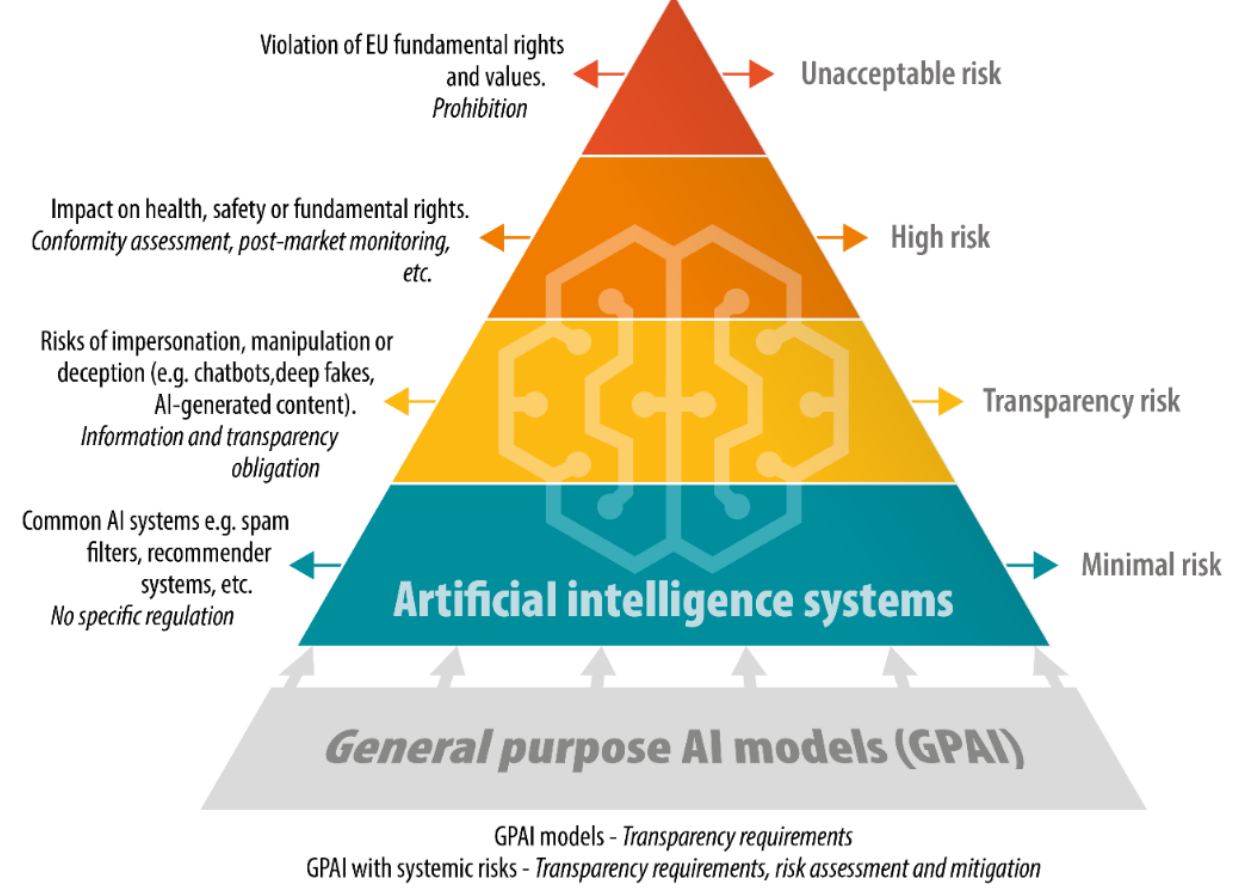
\includegraphics[width=.9\textwidth]{screen2.png} \\

\scriptsize Source: Murphy Figure 1.7
\caption{Fit versus number of parameters of a model}
\label{fig:polynomial_chap11}
\end{figure}

Closely related to flexibility is concept of \emph{degrees of freedom}\index{Degrees of freedom}. In parametric models, the degrees of freedom are defined as the difference between the number of observations and the number of parameters of the model:

\begin{align*}
\operatorname{DF} = n - p
\end{align*}

\noindent Each parameter to be estimated requires one observation and so ''uses up'' one degree of freedom. The model in the bottom left panel of Figure~\ref{fig:polynomial_chap11} has no degrees of freedom left, it has as many parameters $p$ as observations $n$. 

To better understand the concepts of underfitting and overfitting, it is useful to consider the MSE regression loss in more detail. This requires the concepts of expected value and variance of a random variable $X$ from basic statistics.

\begin{infobox}
\paragraph*{Expected Value}\index{Expected value} 
\begin{align*}
E[X] &= \sum_{i=1}^{\infty} x_i p_i \qquad \text{discrete random variable}\\
E[X] &= \int_{-\infty}^{\infty} x p(x) dx \qquad \text{continuous random variable}
\end{align*}
For uniform distributions or unweighted observations $p_i=p_j \; \forall i, j \; $ so that $E[X] = \frac{1}{n} \sum_{i=1}^{\infty} x_i $, i.e. expectation = mean
\end{infobox}

\begin{infobox}
\paragraph*{Variance}\index{Variance!of a random variable} 
\begin{align*}
Var[X] &= E[(X - E[X])^2] = E[X^2] - E[X]^2 
\end{align*}
For zero-centered variables $E[X] = 0$ so that $Var[X] = E[X^2]$
\end{infobox}

Equipped with these concepts, one can rewrite the MSE to decompose it into three parts:

\begin{align*}
\operatorname{MSE} &= E[(y - \hat{f})^2] \\
    & = E [ y^2 - 2 y \hat{f} + \hat{f}^2] \\
    &= E [y^2] - 2E[y\hat{f}] + E[\hat{f}^2]
\end{align*}
\noindent Using the definitions for expected value and variance, each of part of the MSE can be further rewritten:
\begin{align*}
E[\hat{f}^2] &= E[\hat{f}^2] - E[\hat{f}]^2 + E[\hat{f}]^2 \\
             &= Var[\hat{f}] + E[\hat{f}]^2 \\
\\
E[y^2] &= E[(f+\epsilon)^2] \\
       &= E[f^2] + 2E[f \epsilon] + E[\epsilon^2]\\
       &= f^2 + 2f \cdot 0 + \sigma^2 &\qquad (f \text{\, is not random and} \, E[\epsilon] = 0)\\
       &= f^2 + \sigma^2 \\ 
\\
E[y \hat{f}] &= E[(f + \epsilon)\hat{f}] \\
             &= E[f \hat{f}] + E[\epsilon \hat{f}] \\
             &= E[f \hat{f}] + E[\epsilon] E[\hat{f}] \\
             &= E[f \hat{f}] + 0 \cdot E[\hat{f}] \\
             &= f E[\hat{f}] \\
\end{align*}
\noindent Putting this all together, we can rewrite the MSE as follows:
\begin{align*}
MSE &= f^2 + \sigma^2 - 2 f E[\hat{f}] + Var[\hat{f}] + E[\hat{f}]^2 \\
    &= (f - E[\hat{f}])^2 + \sigma^2 + Var[\hat{f}] \\
    &= Bias[\hat{f}]^2 + \sigma^2 + Var[\hat{f}] \\
\end{align*}

The \emph{bias}\index{Bias (in prediction)} of an estimated model $\hat{f}$ expresses how far the expected value of the estimated model $\hat{f}$ is away from the true target value $f$, while the \emph{variance}\index{Variance!of a predictive model} of an estimated model $\hat{f}$ expresses how much the expected value of the estimated model varies with different inputs or data sets. The final part of the MSE is the \emph{irreducible error}\index{Irreducible error} $\sigma^2$ that represents the random variations of the data around the true target value $f$.

An underfitting model\index{Underfitting} will necessarily have a large bias as it is not close to the true model. This was illustrated by the orange line model in Figure~\ref{fig:freedom}. As underfitting models are often models that are too simple, they tend to have small variance, but this is not necessarily true for all models. 

In contrast, overfitting\index{Overfitting} models necessarily have a large variance. Because they are fitted to the idiosyncratic specific values of the training data, they do not generalize well to new, unseen test data. New data, even if it is drawn from the same probability distribution or population, will lead to very different predicted outputs. Thus, a large variance of a model is manifested by a large test error. A severely overfitted model may also have a large bias. An example of this is the overfitted green model in Figure~\ref{fig:freedom}, or the degree 20 polynomial model in Figure~\ref{fig:polynomial_chap11}. Neither of these are close to the true model. 

A well-fitting model is one that does not minimize the bias or the variance but finds the overall optimum by minimizing the joint error. To estimate the variance, it is necessary to apply the model to independent test data. In other words, a well-fitting model is one that minimizes the test error. This central idea is known as the \emph{bias and variance trade-off} and is illustrated in Figure~\ref{fig:biasvariancetradeoff}. Note that the total error also includes the \emph{irreducible error} which cannot be removed but is independent of model complexity.

\begin{figure}
\centering
\centering
\includegraphics[width=.75\textwidth]{bias_variance.png}\\

\scriptsize \url{https://commons.wikimedia.org/wiki/File:Bias_and_variance_contributing_to_total_error.svg}
\caption{Bias and variance trade-off}
\label{fig:biasvariancetradeoff}
\end{figure}

Returning to the characteristics of explanation and prediction, it is now clear that explanation aims to minimize only the bias by seeking to identify the true model. In contrast, prediction also includes a reduction of variance and focuses on minimizing the overall or joint error.

While this section has derived the concepts of bias and variance using regression models, those concepts also apply to classification models. However, the classification loss functions do not lend themselves to the easy separation of the error as the MSE loss function above.

\section{Model Quality in Classification}

In classification models, the primary quality criterion is the \emph{error rate}\index{Error rate}, which can be calculated both for training and for test data as the proportion where the predicted class $\hat{y}_i$ is not the true class $y_i$:

\begin{align*}
\frac{1}{n}\sum^n_{i=1} \Ident(y_i \neq \hat{y}_i)
\end{align*}

\noindent Here, $\Ident(\cdot)$ is the \emph{identity function} that is 1 if its argument is true, 0 otherwise.

Classification methods typically produce as output the probability of an observation belonging to any of $k$ classes. A decision rule is then required to actually classify an observation based on this probability. A \emph{Bayes classifier} assigns each observation to the class $j$ with the highest probability, given its predictor values $x_0$:

\begin{align*}
\argmax_j \Pr(Y=j| X=x_0)
\end{align*}

\noindent Consequently, the error rate can be written as:
\begin{align*}
1 - E \left( \argmax_j \Pr (Y=j | X) \right)
\end{align*}

The most common type of classification is \emph{binary classification}, which assigns observations to one of two classes, e.g. true or false, normal or abnormal, good or bad, zero or one, etc. \emph{Multinomial classification}, also called \emph{multi-class classification} assigns observations to one of more than two classes. This section first considers binary classification before moving to multinomial classification.

A Bayes classifier is an \emph{ideal classifier}. The Bayes classifier\index{Bayes classifier} error rate is the irreducible error and forms the lower bound of practically achievable classification error rates. The Bayes classifier is an ideal classifier because in practice the probabilities of class membership, conditional on the observed predictor values, are unknown and must be estimated from data using a statistical model. However, estimation introduces error.

A simple, non-parametric classifier is the k-Nearest Neighbour (KNN) method\index{k-nearest neighbour!classfication}. This classifier identifies a set of $k$ observations closest to an observation $x_0$ whose class is to be predicted, called the neighbourhood $N_0$. The class membership probabilities are then estimated as the proportions of observations in the neighbourhood that belong to the different classes $j$:

\begin{align*}
\Pr (Y=j|X=x_0) = \frac{1}{K} \sum_{i \in N_0} \Ident (y_i=j) 
\end{align*}

\noindent 
Here, $\Ident(\cdot)$ is the identity function that is 1 if its argument is true, and 0 otherwise.

\begin{figure}
\centering
\includegraphics[width=.75\textwidth]{Figures_Chapters_1-6/Chapter2/2_14.pdf} \\
\vspace{3mm}
\scriptsize Source: ISLR2 Figure 2.14
\caption{KNN example for binary classification}
\label{fig:knn1}
\end{figure}

Figure~\ref{fig:knn1} provides an example for $k=3$. The left panel in this figure shows points for which the classes, blue or orange, are known. When predicting the class for a new point, marked by the ''$\times$'', the three nearest neighbours are identified. Of these, two are blue and one is yellow. Thus, the probability of the new point being yellow is estimated as $1/3$ and that of it being blue is estimated as $2/3$. The Bayes decision rule would classify the new point as blue. The right panel shows the result of classifying a large set of points as blue or yellow. The panel clearly shows the \emph{decision boundary}\index{Decision boundary} of the classifier that separates the predicted class memberships, represented by the black line.

When KNN is used for regression\index{k-nearest neighbour!regression}, the predicted output value is usually estimated as the mean output values of the $k$ neighbours in the neighbourhood $N_0$.

\begin{figure}
\centering
\includegraphics[width=.75\textwidth]{Figures_Chapters_1-6/Chapter2/2_16.pdf} \\
\vspace{3mm}
\scriptsize Source: ISLR2 Figure 2.16
\caption{Decision boundaries of two KNN classifiers}
\label{fig:knn2}
\end{figure}

To show how the KNN classifier behaves as a function of different values for $k$, consider the two panels in Figure~\ref{fig:knn2}. The left panel shows the classifications and the decision boundaries for $k=1$. It also shows the true Bayes boundary as a dashed blue line. The KNN classifier shows relatively low bias in that it its decision boundary is somewhat close to the Bayes decision boundary. However, it also shows signs of overfitting when the classifier decision boundary adapts to various individual points along both sides of the true boundary. The right panel shows a KNN classifier for the same data set with $k=100$. It is clear that the classifier decision boundary does not follow the true decision boundary, that is, the classifier shows high bias. This classifier is underfitted. On the other hand, given that $k=100$, it is not susceptible to individual data points or sampling changes for new data (as long as the new data is generated from the same true model), that is, it shows low variance. 

\begin{figure}
\centering
$\vcenter{\hbox{
\includegraphics[width=.49\textwidth]{Figures_Chapters_1-6/Chapter2/2_17.pdf}}}$ 
$\vcenter{\hbox{\includegraphics[width=.49\textwidth]{Figures_Chapters_1-6/Chapter2/2_15.pdf}}}$ \\

\vspace{3mm}
\scriptsize Source: ISLR2 Figures 2.14, 2.15
\caption{KNN error rates and optimal KNN decision boundary}
\label{fig:knn3}
\end{figure}

In KNN classification (and also in KNN regression), the model with the lower value of $k$ is the more flexible model, and is more likely to lead to overfitting. As $k$ increases, the model becomes less flexible, less likely to overfit, and increasingly more likely to underfit and have a high bias. The left panel in Figure~\ref{fig:knn3} shows the training and test error rates for the KNN classifier for different values of $k$. Note the horizontal axis shows the inverse of $k$, that is $1/k$, larger $k$ are to the left, smaller $k$ are to the right in this panel. The right panel in Figure~\ref{fig:knn3} shows the classifications and decision boundary for $k=10$, which is close to optimal.

\begin{exercisebox}
The table below provides a training data set containing six observations, three predictors, and one qualitative response variable.\\ 
\vspace{.5\baselineskip}
\begin{center}
\footnotesize
\renewcommand{\arraystretch}{1.1}
\begin{tabular}{l|r|r|r|l} \hline
Obs. & $X_1$ & $X_2$ & $X_3$ & $Y$ \\ \hline
1 & 0 & 3 & 0 & Blue \\
2 & 2 & 0 & 0 & Blue \\
3 & 0 & 1 & 3 & Blue \\
4 & 0 & 1 & 2 & Yellow \\
5 & -1 & 0 & 1 & Yellow \\
6 & -1 & 1 & 1 & Blue \\ \hline
\end{tabular}
\end{center}

\vspace{.5\baselineskip}
Suppose we wish to use this data set to make a prediction for $Y$ when $X_1=X_2=X_3=0$ using K-nearest neighbours.
\vspace{.5\baselineskip}
\begin{enumerate}
  \item Compute the Euclidean distance (''L2-norm'' or ''Euclidean norm'' of the vector difference) between each observation and the test point. The L2-norm is the root of the sum of squared differences.
  \item What are your predictions for $K=1$ and for $K=3$? Why?
  \item If the Bayes decision boundary is highly non-linear, would you expect the best value for $K$ to be large or small? Why?
\end{enumerate}

\vspace{.5\baselineskip}\scriptsize Adapted from ISLR Exercise 2.7
\end{exercisebox}

In binary classification, the \emph{confusion matrix}\index{Confusion matrix} is a useful tool for summarizing the performance of a classifier. It tabulates the number of positive and negative predictions that match the true values. The following confusion matrix shows the results of a hypothetical binary classifier for credit card defaults that assigns classes by highest probability:

\begin{center}
\renewcommand{\arraystretch}{1.25}

Decision rule: $\Pr(\text{default=Yes} | X=x) > 0.5$ (Bayes) \\ \vspace{2mm}
\begin{tabular}{cc|cc|c} \hline
     & & \multicolumn{2}{c|}{\emph{True default status}} \\
     & & No & Yes & Total \\ \hline
\emph{Predicted} & No & 9644 & \emph{252} & 9896 \\ 
\emph{default status} & Yes & \emph{23} & 81 & 104 \\ \hline
     & Total & 9667 & 333 & 10000 \\ \hline
\end{tabular} \\
\vspace{\baselineskip}
\scriptsize Source: ISLR2 Table 4.4 \normalsize \\
\end{center}

The overall error rate is $\frac{23 + 252}{10000} = 0.0275 = 2.75\%$. However, of the true defaulters, only $81/333 = 24.3\%$ were correctly predicted. This is called the \emph{recall} or \emph{sensitivity}. It also means that the error rate for the class of true defaulters is a rather high $75.7\%$. The overall error rate remains small mainly because there are very few true defaulters, only $333/10000$. Of the non-defaulters, $9644/9667=99.8\%$ are correctly predicted. This is known as the \emph{specificity}, for an error rate of only $0.02\%$.

While a Bayes classification rule of choosing the highest probability class is easy to justify on probabilistic grounds, practical applications often choose a different \emph{threshold}. In this fictitious example, credit card defaulters may pose a significant risk so that it may be worthwhile reducing the error rate for the true defaulters, even at the the cost of increasing the error rate for the non-defaulters. This is shown in the following confusion matrix:

\begin{center}
\renewcommand{\arraystretch}{1.25}

Decision rule: $\Pr(\text{default=Yes} | X=x) > 0.2$ \\ \vspace{2mm}
\begin{tabular}{cc|cc|c} \hline
     & & \multicolumn{2}{c|}{\emph{True default status}} \\
     & & No & Yes & Total \\ \hline
\emph{Predicted} & No & 9432 & 138 & 9570 \\ 
\emph{default status} & Yes & 235 & 195 & 430 \\ \hline
     & Total & 9667 & 333 & 10000 \\ \hline
\end{tabular} \\
\vspace{\baselineskip}
\scriptsize Source: ISLR2 Table 4.5 \normalsize \\
\end{center}

More of the true defaulters are correctly predicted and the sensitivity has improved to $58.6\%$ while the error rate for true defaulters has been reduced to $51.4\%$. On the other hand, the specificity has decreased to $97.6\%$ and the overall error rate has increased to $3.73\%$. 

In general, a confusion matrix shows four different values, the \emph{true negatives} (TN)\index{True negative}, \emph{true positives} (TP)\index{True positive}, \emph{false negatives} (FN)\index{False negative} and \emph{false positives} (FP)\index{False positive} as shown in the following table:

\begin{center}
\renewcommand{\arraystretch}{1.25}

\begin{tabular}{cc|cc|c} \hline
     & & \multicolumn{2}{c|}{\emph{True class}} \\
     & & No (-) & Yes (+) & Total \\ \hline
\emph{Predicted} & No (-) & True Neg. (TN) & False Neg. (FN) & $N^*$ \\ 
\emph{class} & Yes (+) & False Pos. (FP) & True Pos. (TP) & $P^*$ \\ \hline
     & Total & $N$ & $P$ &  \\ \hline
\end{tabular} \\
\end{center}

From these four values, a number of model quality statistics can be computed. Frequently used are the recall, specificity, precision, accruacy, and F1 score, which are highlighted in the following list:

\begin{itemize}
   \item Sensitivity\index{Sensitivity|see{Recall}}, \textbf{Recall}\index{Recall}, Hit Rate, True Positive Rate:
\begin{align*}
TPR = \frac{TP}{P} = \frac{TP}{TP+FN} = 1 - FNR
\end{align*}
   \item \textbf{Specificity}\index{Specificity}, Selectivity\index{Selectivity|see{Specificity}}, True Negative Rate:
\begin{align*}
TNR = \frac{TN}{N} = \frac{TN}{TN+FP} = 1 - FPR
\end{align*}
   \item \textbf{Precision}\index{Precision!in classification}, Positive Predictive Value:
\begin{align*}
PPV = \frac{TP}{TP+FP} = 1 - FDR
\end{align*}
   \item Negative Predictive Value:
\begin{align*}
NPV = \frac{TN}{TN+FN} = 1 - FOR
\end{align*}
   \item Miss Rate, False Negative Rate:
\begin{align*}
FNR = \frac{FN}{P} = \frac{FN}{FN + TP} = 1 - TPR
\end{align*}
   \item Fall-out, False Positive Rate:
\begin{align*}
FPR = \frac{FP}{N} = \frac{FP}{FP+TN} = 1 - TNR
\end{align*}
   \item False Discovery Rate:
\begin{align*}
FDR = \frac{FP}{FP+TP} = 1 - PPV
\end{align*}
   \item False Omission Rate:
\begin{align*}
FOR = \frac{FN}{FN+TN} = 1 - NPV
\end{align*}
   \item \textbf{Accuracy}\index{Accuracy (in classification)} (= 1 - Error Rate):
\begin{align*}
ACC = \frac{TP+TN}{P+N} = \frac{TP + TN}{TP + TN + FP + FN}
\end{align*}
   \item \textbf{F1 Score}\index{F1 score} (harmonic mean of precision and recall):
\begin{align*}
F1 = 2 \times \frac{PPV \times TPR}{PPV + TPR} = \frac{2 TP}{2TP + FP + FN}
\end{align*}
   \item False Discovery Rate:
\begin{align*}
FDR = \frac{FP}{FP+TP} = 1 - PPV
\end{align*}
   \item False Omission Rate:
\begin{align*}
FOR = \frac{FN}{FN+TN} = 1 - NPV
\end{align*}
\end{itemize}

The above example demonstrated that the true positive rate and the false positive rate (or the true negative rate and false negative rate) are not independent of each other. Generally, increasing the true positive rate will also increase the false positive rate, because one is overall more likely to conclude that an observation is the true class (by adjusting the probability threshold). This suggests that a graph of the true positive rate against the false positive rate as shown in Figure~\ref{fig:roc} can summarize the classifier performance and allows the user to pick a desirable combination of true and false positive rates. The graph in Figure~\ref{fig:roc} is called a \emph{Receiver Operating Characteristics}\index{Receiver operating characteristic}\index{ROC|see{Receiver operating characteristic}} chart, or ROC chart for short. The terminology stems from early experiments with aircraft detection through radar during the 2nd world war. As shown in the figure, a random classifier is characterized by a diagonal line, and good classifiers have curves towards the upper left. Thus, the classifier shown in the green line dominates the one in the orange line, and is in turn dominated by the one represented by the blue line. All three perform better than a random classifier.

\begin{figure}
\centering
\includegraphics[width=.5\textwidth]{roc.png}
\scriptsize \url{https://commons.wikimedia.org/wiki/File:Roc_curve.svg}
\caption{ROC curves of three example classifiers}
\label{fig:roc}
\end{figure}

Because the ROC curve of a perfect classifier runs though the top-left corner of the ROC chart, it is natural to define the overall performance of classifier for various combinations of true and false positive rate by the area under the curve. This also allows easy comparisons of classifiers that do not dominate one another, i.e. whose ROC lines cross each other. The \emph{area-under-the-curve}, or AUC\index{Area under curve}\index{AUC|see{Area under curve}} for short, summarizes the classifier performance in a single number. For the classifier in Figure~\ref{fig:auc}, the AUC is $0.834$, indicated by the green and read areas. A random classifier has an AUC of $0.5$ and a perfect classifier has an AUC of $1$. 

\begin{figure}
\centering
\includegraphics[width=.65\textwidth]{auc.png}
\scriptsize \url{https://commons.wikimedia.org/wiki/File:ROC_curve_example_highlighting_sub-area_with_low_sensitivity_and_low_specificity.png}

\caption{AUC of an example classifier}
\label{fig:auc}
\end{figure}

\begin{exercisebox}
Consider the two confusion matrices above. 
  \begin{itemize}
     \item Compute precision and recall for the two confusion matrixes above
     \item Computer accuracy and F1 values for the two confusion matrixes above
     \item The two confusion matrixes above characterize two points on the ROC curve. Plot the two points for this classifier in an ROC space/diagram. Are they above or below the diagonal?
  \end{itemize}
\end{exercisebox}

\begin{exercisebox}
Consider a medical testing scenario where 1000 individuals are tested for a disease. The results are:
  \begin{itemize}
    \item 100 people actually have the disease, and 900 do not.
    \item Out of the 100 people with the disease, 90 are correctly identified as having it, but 10 are not detected.
    \item Of the 900 people without the disease, 810 are correctly identified as not having it, but 90 are incorrectly identified as having the disease.
  \end{itemize}
  Calculate the precision, recall, sensitivity, and accuracy of the test. \\
  \emph{Tip}: Write down the confusion matrix first.
\end{exercisebox}

\begin{exercisebox}
Given the following results from a machine learning model:
  \begin{itemize}
    \item Precision: 0.75
    \item Recall: 0.60
    \item Accuracy: 0.80
  \end{itemize}
Answer the following questions:
  \begin{enumerate}
    \item What percentage of identified positives are actually positive?
    \item What percentage of actual positives are identified by the model?
    \item What percentage of the total classifications were correct?
  \end{enumerate}
\end{exercisebox}

\begin{exercisebox}
Consider a binary classification task with the following confusion matrix at a certain threshold:
  \begin{itemize}
    \item TP: 150, FP: 50
    \item FN: 30, TN: 200
  \end{itemize}
  Discuss how adjusting the classification threshold might affect precision, recall, and accuracy. What happens if the threshold is increased or decreased?
\end{exercisebox}

\section{Multinomial Classification}

Multinomial or multi-class classification assigns each observation to one of more than two classes. In this setting, the confusion matrix becomes larger, as shown in the following example, where the overall accuracy is calculated as the sum of the diagonal element divided by the sum of all elements, i.e. sum(diag(.)) / sum(.) $=17/24=.71$.

\begin{center}
\vspace{\baselineskip}
\renewcommand{\arraystretch}{1.1}

\begin{tabular}{cc|ccc|l} \hline
     & & \multicolumn{3}{c|}{\emph{True class}} \\
                 &   & 0 & 1 & 2 & Prob \\ \hline
\multirow{3}{1.1cm}{\emph{Predicted Class}} & 0 & 4 & 2 & 0 & $q_0 = 6/24  = .25$ \\ 
                 & 1 & 1 & 5 & 2 & $q_1 = 8/24  = .33$ \\
                 & 2 & 2 & 0 & 8 & $q_2 = 10/24 = .42$ \\ \hline
     & Prob & $p_0$ & $p_1$ & $p_2$ &  \\
     &      & $=7/24$ & $=7/24$ & $=10/24$ &  \\ 
     &      & $=.29$ & $=.29$ & $=.42$ &  \\ \hline
\end{tabular} \\
\vspace{\baselineskip}
\end{center}

While the concept of a confusion matrix remains applicable, it is not immediately obvious what the true negative, true positive, false negative, and false positive values are.  One way to overcome this is to reduce the classification results to a binomial case by treating each class in turn as the ''positive class'' and all others as ''negative''. This is called ''one-versus-rest'' (OvR), ''one-versus-all'' (OvA), or ''one-against-all'' (OaA). 

In \emph{micro-averaging}\index{Micro averaging}, the TP, TN, FP, and FN values are counted for all classes using OvR, and then summed. These total TP, TN, FP, and FN values are then used to compute precision, recall and other metrics. This gives equal weight to each instance but may overemphasize the classification for a dominant majority class. Importantly, for micro-averaging, precision equals recall equals accuracy.

In \emph{macro-averaging}\index{Macro averaging}, the TP, TN, FP, and FN values are counted for all classes, but instead of summing these values, precision and recall are calculated for each class. These precision and recall values are then averaged over all classes, optionally weighting each class by its true count of instances. Macro-averaging is appropriate when all classes are equally important. It is also appropriate for an imbalanced data set and ensures that all classes contribute equally. However, it may mask poor performance of important minority classes, and it may lower overall performance measures due to low classifier performance on small or unimportant classes that nonetheless contribute equally to larger or important classes. 

\begin{exercisebox}
For the multi-class confusion matrix above,
\begin{enumerate}
  \item Compute precision and recall for each class.
  \item Compute the micro-averages of precision and recall and show that they equal the accuracy.
  \item Compute the macro-averages of precision and recall.
\end{enumerate}
\end{exercisebox}

While precision, recall, and accuracy are useful metrics for evaluating a binary or multinomial classifer, they do not lend themselves to be used directly as loss functions in fitting a model. This is because the assignment of an observation to a class is a function of the probability of its class membership and the actual class assignment may depend on the chosen threshold probability or other decision rule. Thus, a desirable loss function is a function that expresses how close or how different the predicted class membership probabilities are from the true class membership probabilities. 

There are two commonly used metrics that quantify such a difference. Both have their origin in information theory and the two are closely related to each other. First, the \emph{cross-entropy}\index{Cross-entropy} of two probability distributions $p_i$ and $q_i$ over the same set of classes $i$ is defined as:

\begin{align*}
H(p, q) = - \sum_i p_i \log q_i \qquad \text{Cross-entropy}
\end{align*}

\noindent Here, $p_i$ is the true probability of belonging to class $i$ whereas $q_i$ is the predicted probability of belonging to class $i$. The cross-entropy captures the similarity or difference of the two probability distributions.

The second metric is the \emph{Kullback-Leibler (KL) divergence}\index{Kullback-Leibler divergence}\index{KL divergence|see{Kullback-Leibler divergence}}. It is effectively the cross-entroy minus the entropy of the true probability distribution, as the following derivation shows:

\begin{align*}
D_{KL}(P || Q) &= \sum_i p_i \log \left( \frac{p_i}{q_i} \right) \qquad \text{Kullback-Leibler (KL) divergence}\\
  & = \sum_i p_i \log p_i - \sum_i p_i \log q_i \\
  & = - H(p, p) + H(p, q)
\end{align*}

\begin{exercisebox}
Consider the two probability distributions $P$ and $Q$ in the following diagrams. \begin{center}
\includegraphics[width=.5\textwidth]{kl.png}

\tiny \url{https://commons.wikimedia.org/wiki/File:Kullback-Leibler_distributions_example_1.svg}
\normalsize
\end{center}

%\vspace{3mm}
\begin{enumerate}
   \item Calculate the cross-entropy of P and Q.
   \item Calculate the entropy of P.
   \item Calculate the KL divergence of P and Q.
\end{enumerate}

\vspace{\baselineskip}
\emph{Tip}: Binomial distribution: $\Pr(P=k) = \frac{n!}{k!(n-k)!} p^k (1-p)^{n-k}$ \\
\end{exercisebox}

\begin{exercisebox}
Calculate the cross-entropy and KL-divergence for the multi-class confusion matrix above.
\end{exercisebox}

\begin{exercisebox}
Given two probability distributions P and Q over a discrete set of events, where $P = [0.1, 0.4, 0.5]$ and $Q = [0.2, 0.3, 0.5]$, calculate the cross-entropy $H(P, Q)$ and the KL-divergence $D_{KL}(P || Q)$.
\end{exercisebox}

\begin{exercisebox}
In a binary classification task, you have the following probability distributions for the actual labels (P) and predicted labels (Q):
\begin{itemize}
  \item P = [1, 0] (the actual class is positive)
  \item Q = [0.7, 0.3] (the model predicts a 70\% chance of being positive)
\end{itemize}
Calculate the cross-entropy loss for this scenario.
\end{exercisebox}

\begin{exercisebox}
Calculate the KL divergence between the following probability distributions:
  \begin{itemize}
     \item P = [0.1, 0.9]
     \item Q = [0.5, 0.5]
  \end{itemize}
\end{exercisebox}

\section{Crossvalidation Methods}

Recall that the goal in prediction is to have an unbiased assessment of the true classification or regression error, and to generalize to prediction of future, yet unseen observations. Finding a suitable prediction model involves two separate steps, that of \emph{model selection}, and that of \emph{model assessment}. Model selection estimates the predictive performance, that is, the error or loss, of different models in order to choose the best one. After having chosen the final model, its prediction error must again be estimated on new data. This is to avoid model selection capitalizing on specific idiosyncrasies of the test data, which may not hold for new, as yet unseen data\index{Cross-validation}.

The \emph{validation set approach}, or ''holdout'' method\index{Holdout sample}, then requires not only a training and test data set, but a third set, the validation set. The training data is used to train each of a set of candidate models, the validation data is used to test each candidate model, and the test data is used to evaluate the finally selected model. Typically, the data set is randomly split into 50\% training data, 25\% validation data, and 25\% test data, but other splits are used as well. 

One potential problem with this approach is that the validation error can be highly variable and depends critically on the way the data is split. One random split can show very different characteristics than another random split. A second potential problem is that the validation error may overestimate the actual error, because the training set is small, only half of the full data set. Figure~\ref{fig:holdout} illustrates the first problem. A single split of the data results in the validation error shown in the left panel. However, repeating the random splitting ten times results in ten different validation errors that may be very different from each other, as shown in the right panel of that figure.

\begin{figure}[b]
\centering 

\includegraphics[width=.9\textwidth]{Figures_Chapters_1-6/Chapter5/5_2.pdf}
\scriptsize Source: ISLR2 Figure 5.2
\caption{Validation error for different random splits of a data set}
\label{fig:holdout}
\end{figure}

One way to deal with both problems is to use \emph{leave-one-out cross-validation} (LOOCV)\index{Leave-one-out cross-validation}\index{LOOCV|see{Leave-one-out cross-validation}}. In LOOCV, each observation is designated as test observation in turn, while the remaining $n-1$ observations form the training data set. The model is trained on the training data and tested on the single test observation. This procedure is repeated $n$ times as each observation becomes the test observation in turn. The cross-validation error is simply the mean of the $n$ training errors:

\begin{align*}
CV = \frac{1}{n} \sum\nolimits_{i=1}^n \operatorname{Err}_i
\end{align*}

The advantage to LOOCV is that it addresses the two potential problems with the holdout sample approach. Additionally, it is deterministic as there is no randomness to the resulting validation error estimate, because there are no random splits of the data set. Finally, LOOCV shows less overstimation of the validation error rate than the holdout approach. However, a significant drawback is that this approach is computationally expensive, because the model must be fit or trained $n$ times to $n$ different training data sets. 

As a compromise between the holdout sample approach and LOOCV, business analysts often use \emph{k-fold cross-validation}\index{k-fold cross-validation}. In this approach, the data set is randomly divided into $k$ sub-samples (''folds''). Each fold is selected as the test data set in turn, with the remaining $k-1$ folds combining to form the training data set. The cross-validation error is simply the mean of the $k$ cross-validation errors for each of the $k$ test folds. Typically, $k$ is chosen as $5$ or $10$.

\begin{align*}
CV = \frac{1}{k} \sum\nolimits_{i=1}^k \operatorname{Err}_i
\end{align*}

k-fold cross-validation is computationally less expensive and less stable than LOOCV, but it is more stable than the holdout sample approach. The k-fold cross-validation error estimate has a higher bias but lower variance than that of LOOCV. Figure~\ref{fig:kfold} illustrates the stability. The left panel shows the LOOCV error estimate for a regression number with different degrees of polynomials. The right panel shows ten different runs each of 10-fold cross-validation (i.e. the model was trained a total of 100 times). The 10-fold cross-validation errors show a much smaller variation than the different holdout sample errors in Figure~\ref{fig:holdout}.

\begin{figure}
\centering

\includegraphics[width=\textwidth]{Figures_Chapters_1-6/Chapter5/5_4.pdf}
\scriptsize Source: ISLR2 Figure 5.4
\caption{Cross-validation error with LOOCV and 10-fold cross-validation}
\label{fig:kfold}
\end{figure}

One important consideration in splitting the data is preventing \emph{information leakage}\index{Information leakage} from training to test or validation data set, in order to ensure that the test and validation data sets are truly independent of the training data. One way in which information could be leaked is when selection of input variables or predictors is done based on characteristics of the entire data set, for example the variance of a variable or the correlation between variables in the entire data set. This selection affects both the training and the test data, essentially leaking some information from the training data to the test data, and thereby making the test data set not truly independent. Another way in which information can leak is by pre-processing variables, like centering around the mean or scaling them to have unit variance. When this is based on the mean or variance of the full data set, information from the training set leaks to the test or validation set, making those data sets not fully independent. As a general rule, any predictor or feature selection and data pre-processing must be done independently for each training set, \emph{after} the split or splits (in the case of k-fold CV) have been made. 

\section{Review Questions}
\paragraph*{Supervised and unsupervised learning}
\begin{enumerate}[nosep]
    \item Explain the difference between supervised and unsupervised learning. Provide an example for each.
    \item Define regression and classification. Discuss one real-life application for each.
\end{enumerate}
\paragraph*{Parametric methods}
\begin{enumerate}[nosep,resume*]
    \item What is the difference between a parametric and a non-parametric machine learning model? Provide examples.
    \item What are some of the key metrics used to evaluate the quality of a regression model versus a classification model? Discuss their relevance in real-world applications.
\end{enumerate}
\paragraph*{Explanation and prediction}
\begin{enumerate}[nosep,resume*]
    \item Define the terms \emph{explanation} and \emph{prediction}. How do they differ in their core objectives when using statistical models?
    \item Explain what is meant by the statement that explanatory models are intended to be isomorphic to causal processes.
    \item Discuss why explanation models focus on bias minimization and how this affects the model design and interpretation.
    \item Provide examples where an explanation model would be more suitable than a prediction model, and vice versa.
    \item What are the implications of using a predictive model that does not represent the true causal relationship but still produces accurate predictions?
\end{enumerate}
\paragraph*{Bias and variance}
\begin{enumerate}[nosep,resume*]
    \item Explain the terms \emph{bias} and \emph{variance} in the context of statistical modeling. How do they relate to the goals of prediction?
    \item Explain the bias-variance tradeoff with an example. You may use a simple regression model as a reference.
    \item What are overfitting and underfitting in the context of machine learning? How can each be detected and mitigated?
    \item Describe a scenario where a high-bias model would be more appropriate than a low-bias model.
    \item Given the following scenarios, identify whether the model is likely suffering from high bias, high variance, or is well-balanced:
	\begin{itemize}
	  \item A model that performs well on training data but poorly on unseen test data.
	  \item A simple linear regression model that is unable to capture the complexities of the data, resulting in poor performance on both training and test data.
	  \item A model that performs equally well on training and test data.
	\end{itemize}
    \item Describe techniques to reduce bias in a machine learning model.
    \item Given a dataset where the relationship between features and target is non-linear and complex, propose a strategy to improve a model that initially has high bias (e.g., linear regression).
    \item List and explain strategies to reduce variance in a machine learning model.
    \item Imagine you have a deep learning model that performs exceptionally well on the training data but poorly on the validation data. What steps would you take to address this issue?
\end{enumerate}
\paragraph*{Regression evaluation}
\begin{enumerate}[nosep,resume*]
    \item Explain the difference between Mean Squared Error (MSE) and Mean Absolute Error (MAE). Why is MAE considered more robust to outliers?
    \item Describe the Huber loss function and discuss its advantages over MSE and MAE.
    \item Discuss the significance of using test data to evaluate the quality of a regression model. Why is it not advisable to rely solely on training data for model evaluation?
\end{enumerate}
\paragraph*{KNN classification}
\begin{enumerate}[nosep,resume*]
    \item Explain how the KNN algorithm estimates the class of a new observation. Include a discussion on the effect of the choice of \( k \).
    \item How does changing the value of \( k \) in the KNN classifier affect the bias and variance of the model?
\end{enumerate}
\paragraph*{Binary classification evaluation}
\begin{enumerate}[nosep,resume*]
    \item Define the terms ''precision'' and ''recall''. Provide a scenario where a high recall is more important than high precision, and vice versa.
    \item Describe the following metrics and explain their importance in the evaluation of classification models:
    \begin{itemize}
        \item Precision
        \item Recall (Sensitivity)
        \item F1 Score
        \item Specificity
    \end{itemize}
    \item Discuss the importance of the ROC curve and AUC in the evaluation of classification models. How do these metrics help in assessing the performance of a model?
    \item Given a scenario where you are developing a classifier for a medical diagnosis application, which metric would you prioritize and why?
\end{enumerate}
\paragraph*{Multinomial classification evaluation}
\begin{enumerate}[nosep,resume*]
    \item Explain what is meant by multinomial classification. How does it differ from binary classification?
    \item Describe the purpose and structure of a confusion matrix in the context of multinomial classification.
    \item How is the overall accuracy calculated using a confusion matrix for multinomial classification? Explain using an example.
    \item Discuss the difference between micro-averaging and macro-averaging in the context of evaluating classification models.
\end{enumerate}
\paragraph*{Cross-entropy and KL-divergence}
\begin{enumerate}[nosep,resume*]
  \item Define cross-entropy and explain its significance in machine learning, especially in classification tasks.
  \item Define Kullback-Leibler divergence and explain its relationship with cross-entropy.
\end{enumerate}
\paragraph*{Cross-validation}
\begin{enumerate}[nosep,resume*]
    \item Explain the concept of cross-validation and how it helps in model assessment.
    \item What is the validation set approach in model evaluation? Describe its potential drawbacks.
    \item How does the validation set approach help mitigate the risk of model overfitting?
    \item Describe the leave-one-out cross-validation (LOOCV) method. What are the benefits and limitations of using LOOCV for model validation?
    \item Compare and contrast LOOCV with the traditional holdout method. In what scenarios might LOOCV be particularly beneficial?
    \item Explain k-fold cross-validation. How does it differ from LOOCV in terms of error estimation?
    \item Discuss the impact of the number of folds in k-fold cross-validation on the bias and variance of the model error estimate.
    \item Define information leakage in the context of data splitting for model evaluation. Why is it important to prevent it?
    \item Provide guidelines or methods to prevent information leakage during the preprocessing and feature selection stages of model development.
\end{enumerate}
